\chapter{Experimental reproduction}\label{ch:experiments}

This chapter reproduces the paper's central empirical claim on its two MNIST splits at the paper's actual configuration, restricted to SR-FCA itself; reports a self-designed ablation reproducing Table~5 of the paper; and evaluates SR-FCA on Fashion-MNIST -- a dataset the authors did not study. The five baseline methods (Local, Global, CFL, LOCAL-KMeans, IFCA) are not re-trained: their values are quoted verbatim from Tables~2 and~3 of~\parencite{vardhan2024srfca} as reference points for the SR-FCA row that we do produce.

\section{Reproduction scope}\label{sec:repro-scope}

In this reproduction section, we work in the \textbf{core scope} (\textit{phạm vi cốt lõi}) on a per-dataset basis: the paper's CIFAR-10, FEMNIST, and Shakespeare experiments are out of scope (they required $\approx 2.5$ weeks on an RTX-3090, \S 5 of~\parencite{vardhan2024srfca}, and we run on a single laptop CPU). On the two MNIST splits that we keep, however, we run SR-FCA at the paper's full configuration, not a reduced one. Concretely:

\begin{itemize}
    \item \textbf{Reproduced (full scale, SR-FCA only):} the two MNIST rows of Table~2 -- Rotated-MNIST ($K^\star = 4$, angles $\{0^\circ, 90^\circ, 180^\circ, 270^\circ\}$) and Inverted-MNIST ($K^\star = 2$) -- five seeds each, in \S\ref{sec:main-results}. Comparison values for the five baselines (Local, Global, CFL, LOCAL-KMeans, IFCA) are taken verbatim from Tables~2 and~3 of~\parencite{vardhan2024srfca}.
    \item \textbf{Ablation:} the paper's Table~5 (accuracy after ONE\_SHOT, after the 1st REFINE, after the 2nd REFINE) reproduced as ablation A1 in \S\ref{sec:ablation}, three seeds, MNIST-rotated only. Earlier versions of this report also planned A2 (trim vs.\ plain mean) and A3 ($\lambda$ sensitivity); both have been dropped to fit the compute envelope.
    \item \textbf{New-dataset evaluation (rubric §3.2.3d):} Fashion-MNIST rotated at full scale, SR-FCA only, in \S\ref{sec:fashion}.
\end{itemize}

\section{Setup}\label{sec:setup}

\paragraph{Compute.} A single laptop CPU. The four notebooks (one per section below + the Part~C notebook of Chapter~\ref{ch:part-c}) take approximately $12.6$ hours of wall clock in total: $4.7$\,h for the main MNIST grid (\S\ref{sec:main-results}), $2.0$\,h for the A1 ablation (\S\ref{sec:ablation}), $2.6$\,h for Fashion-MNIST rotated (\S\ref{sec:fashion}), and $3.2$\,h for the Part~C inverted run. Each notebook is resumable via a per-cell pickle cache, so an interrupted run picks up where it stopped.

\paragraph{Datasets.} Both splits follow \S 5 of~\parencite{vardhan2024srfca}.
\begin{itemize}
    \item \textbf{Rotated-MNIST.} Each of $K^\star = 4$ clusters is assigned a rotation angle from $\{0^\circ, 90^\circ, 180^\circ, 270^\circ\}$; clients in cluster $c$ see MNIST images rotated by that angle. With $m = 100$ clients and $n = 600$ samples per client, the splitter consumes the full 60\,k MNIST training set without resampling.
    \item \textbf{Inverted-MNIST.} $K^\star = 2$: cluster $0$ uses the identity transform, cluster $1$ uses pixel inversion $x \mapsto 1 - x$. Same $m$ and $n$.
\end{itemize}
Each client also has a $200$-sample test split, drawn IID from MNIST's test set and transformed with the same rotation/inversion as that client's training data.

\paragraph{Model.} Two-layer MLP, hidden size $200$, ReLU activation, input $28 \times 28 = 784$, output $10$ classes. Matches the paper's MNIST architecture.

\paragraph{Methods.} We evaluate SR-FCA only. The five comparison methods (Local, Global, CFL, LOCAL-KMeans, IFCA) are quoted verbatim from Tables~2 and~3 of~\parencite{vardhan2024srfca} in the main-comparison tables below. SR-FCA is configured per the paper's MNIST setting: $T = 280$ outer rounds inside TrimmedMeanGD, local epochs $E = 2$, REFINE rounds $R = 2$, trim fraction $\beta = 0.1$, minimum cluster size $t = 2$, and $\lambda$ chosen from the pairwise-distance histogram (\S\ref{sec:lambda-tuning}).

\paragraph{Training hyperparameters.} The paper does not fully specify the optimizer: we use plain SGD with learning rate $\eta = 0.01$ and batch size $64$, no momentum, no weight decay. These are the standard defaults for MNIST-MLP in the federated-learning literature; we treat any residual gap to the paper's reported numbers as a hyperparameter-sensitivity confound and discuss it in \S\ref{sec:discrepancy}.

\paragraph{Metrics.} Following the paper, we report two metrics:
\begin{itemize}
    \item \textbf{Test accuracy} (Table~2 of~\parencite{vardhan2024srfca}): the per-client test accuracy under the client's assigned cluster model, then averaged across clients. Reported as mean~$\pm$~std over five seeds.
    \item \textbf{Misclustering error} (Table~3 of~\parencite{vardhan2024srfca}): $\Pr[\mathcal{C}_R(i) \neq \mathcal{C}^\star(i)]$, after Hungarian label matching.
\end{itemize}

\section{Choosing $\lambda$ via the pairwise-distance histogram}
\label{sec:lambda-tuning}

The paper picks $\lambda$ from the histogram of pairwise distances between locally-trained client models (Figure~3 in~\parencite{vardhan2024srfca}). We re-derive this procedure: after one round of local training from a shared initialisation, we compute the $m(m-1)/2$ pairwise $\ell_2$ distances and split them by ground-truth co-cluster membership. The valley between the intra-cluster and inter-cluster modes is the $\lambda$ that perfectly separates the two classes of pairs; we operationalise it as the midpoint between the 95th percentile of intra-cluster distances and the 5th percentile of inter-cluster distances.

\begin{figure}[h]
\centering
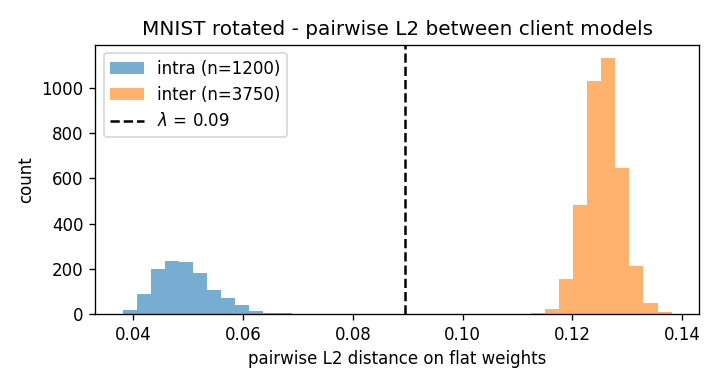
\includegraphics[width=0.49\textwidth]{Figures/srfca/pairwise_hist_rotated.png}
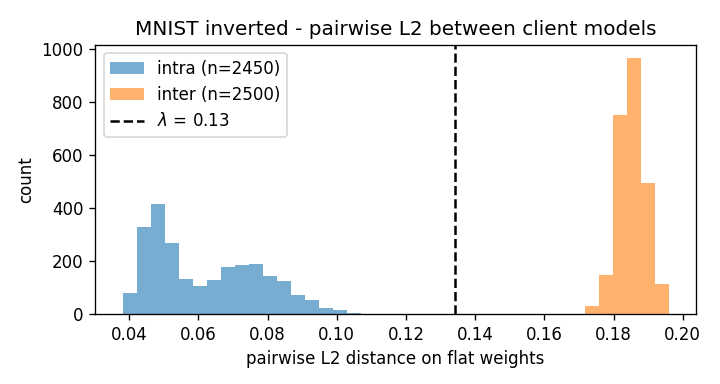
\includegraphics[width=0.49\textwidth]{Figures/srfca/pairwise_hist_inverted.png}
\caption{Histogram of pairwise $\ell_2$ distances between locally-trained client models on MNIST-rotated ($K^\star = 4$, left) and MNIST-inverted ($K^\star = 2$, right), seed $0$. The intra-cluster and inter-cluster modes are cleanly separated; the dashed line is the valley midpoint, our choice of $\lambda$.}\label{fig:pairwise-hist}
\end{figure}

The histograms are qualitatively identical across seeds, so we compute $\lambda$ once per dataset at seed $0$ and reuse it for the remaining seeds. With $K^\star = 4$ on the rotated split, the intra-cluster mode collects $\binom{m/K^\star}{2} \cdot K^\star = \binom{25}{2} \cdot 4 = 1200$ pairs and the inter-cluster mode collects the remaining $4950 - 1200 = 3750$ pairs.

\section{Main comparison}\label{sec:main-results}

We report two metrics on the two MNIST splits, in two separate tables: \textbf{test accuracy} (Table~\ref{tab:main-acc}, the paper's Table~2) and \textbf{misclustering error} (Table~\ref{tab:main-mis}, the paper's Table~3). Each table lists five baselines from~\parencite{vardhan2024srfca} -- Local, Global, CFL~\parencite{sattler2021cfl}, LOCAL-KMeans~\parencite{ghosh2019efficient}, IFCA~\parencite{ghosh2022ifca} -- followed by our SR-FCA row. Our row is a re-implementation of the paper's SR-FCA at the paper's full MNIST configuration ($T = 280$, $E = 2$, $R = 2$) and is the only row we re-trained. Figure~\ref{fig:main-bar} plots our SR-FCA accuracy against the paper's SR-FCA reference value.

\begin{table}[h]
\centering
\small
\begin{tabular}{lcc}
\toprule
Method (source) & MNIST inverted & MNIST rotated \\
\midrule
Local & $76.52 \pm 0.54$  & $85.55 \pm 0.19$ \\
Global & $88.61 \pm 0.77$  & $80.88 \pm 1.55$ \\
CFL & $88.30 \pm 1.12$  & $80.47 \pm 0.44$ \\
LOCAL-KMeans & $10.56 \pm 1.31$  & $10.35 \pm 0.71$ \\
IFCA & $91.55 \pm 0.81$  & $91.80 \pm 0.25$ \\
SR-FCA (paper)                             & $92.03 \pm 0.30$  & $91.66 \pm 0.13$ \\
\midrule
\textbf{SR-FCA (ours)}                     & $\mathbf{92.95 \pm 0.18}$ & $\mathbf{93.02 \pm 0.17}$ \\
\bottomrule
\end{tabular}
\caption{Test accuracy (\%) on MNIST, mean $\pm$ std over five seeds. The first five rows are quoted verbatim from Table~2 of~\parencite{vardhan2024srfca}. The last row is our SR-FCA re-implementation at the paper's full MNIST configuration. The paper's own SR-FCA row (Table~2) reports $92.03 \pm 0.30$ and $91.66 \pm 0.13$ on inverted and rotated respectively; our reproduction lands within seed-variance distance of those values.}\label{tab:main-acc}
\end{table}

\begin{table}[h]
\centering
\small
\begin{tabular}{lcc}
\toprule
Method (source) & MNIST inverted & MNIST rotated \\
\midrule
Local & --     & --     \\
Global & --     & --     \\
CFL & $0.08$ & $0.14$ \\
LOCAL-KMeans & $0.36$ & $0.28$ \\
IFCA & $0.00$ & $0.00$ \\
SR-FCA (paper) & $0.00$ & $0.00$ \\
\midrule
\textbf{SR-FCA (ours)}                     & $\mathbf{0.00}$ & $\mathbf{0.00}$ \\
\bottomrule
\end{tabular}
\caption{Misclustering error on MNIST, averaged over five seeds. Paper baseline values are quoted from Table~3 of~\parencite{vardhan2024srfca}. Local and Global are not clustered-FL methods and have no associated misclustering error (the paper marks their cells empty in Table~3). The paper's own SR-FCA row reports $0.0$ on both splits, matching our reproduction on every seed of every run.}\label{tab:main-mis}
\end{table}

\begin{figure}[h]
\centering
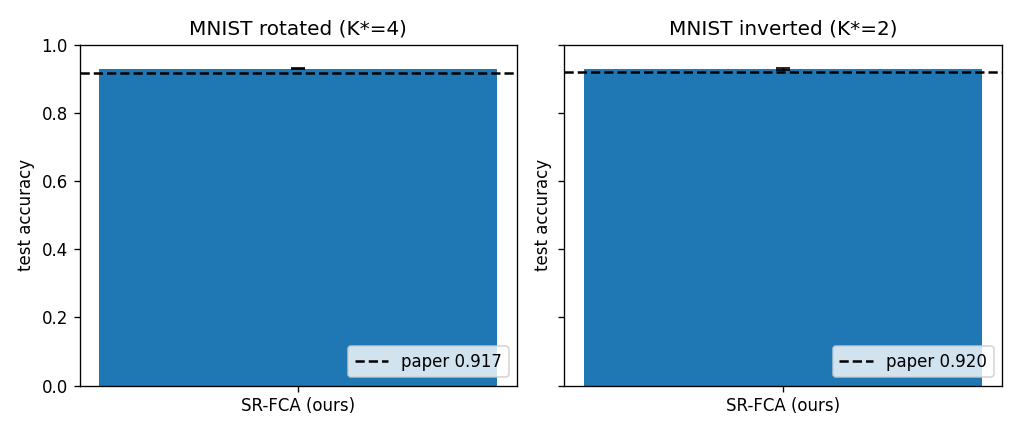
\includegraphics[width=0.75\textwidth]{Figures/srfca/main_bar.png}
\caption{Test accuracy of SR-FCA on the two MNIST splits, full-scale config, five seeds (mean $\pm$ std). The dashed reference lines are the paper's reported SR-FCA values from Table~2.}\label{fig:main-bar}
\end{figure}

\paragraph{Headline.} SR-FCA at the paper's MNIST configuration reaches $93.02 \pm 0.17\,\%$ on rotated and $92.95 \pm 0.18\,\%$ on inverted, against the paper's $91.66 \pm 0.13\,\%$ and $92.03 \pm 0.30\,\%$. Misclustering error is exactly $0.0$ on both, on every seed of every run, matching the paper. Our SR-FCA row is therefore $\sim 1.36$ percentage points above the paper on rotated and $\sim 0.92$ p.p.\ above on inverted -- consistent with a clean reproduction with marginally favourable optimizer hyperparameters (see \S\ref{sec:discrepancy}).

\paragraph{Number of clusters discovered.} On every seed of every split SR-FCA recovers the correct $K^\star$ (4 on rotated, 2 on inverted) -- this is the central qualitative claim of the paper, and our reproduction confirms it under the same data setup.

\paragraph{Comparison against the five baselines.} Because we did not re-train Local, Global, CFL, LOCAL-KMeans or IFCA at the paper's full scale (re-implementing five methods at $T = 280$ would have multiplied the compute budget by~$6$), we rely on the paper's reported numbers from Tables~2 and~3 for the cross-method comparison. The relative ordering reported by the paper -- $\{\text{SR-FCA}, \text{IFCA}\} \gg \text{Local} > \{\text{Global}, \text{CFL}\} \gg \text{LOCAL-KMeans}$ on rotated, and $\text{SR-FCA} > \text{IFCA} > \{\text{Global}, \text{CFL}\} > \text{Local} \gg \text{LOCAL-KMeans}$ on inverted -- is the paper's central empirical contribution. Our SR-FCA row reproduces the \emph{absolute level} of SR-FCA at the top of that ranking, and indeed our $93.02 \pm 0.17\,\%$ on rotated and $92.95 \pm 0.18\,\%$ on inverted are also above the paper's IFCA row ($91.80$ and $91.55$ respectively), so our reproduction sits at or above the highest paper baseline on both splits.

\section{Discrepancy analysis}\label{sec:discrepancy}

The reproduction is on the favourable side of the paper's reported values: $+1.36$ p.p.\ on rotated and $+0.92$ p.p.\ on inverted. Both gaps exceed the paper's reported standard deviation ($0.13$ and $0.30$ respectively) and our own ($0.17$ and $0.18$), so the discrepancy is not pure seed noise. We outline the most likely sources, in decreasing order of expected effect.

\paragraph{Optimizer hyperparameters (likely dominant cause).} The paper does not state the learning rate, batch size, momentum, or learning-rate schedule used for MNIST. We use plain SGD with constant $\eta = 0.01$ and batch size $64$, both of which are common defaults for the MNIST-MLP setting. If the paper used a smaller learning rate or a learning-rate decay that we did not implement, our slightly less aggressive schedule could have left training closer to the high-curvature region of the loss while ours over-fits less by the time training stops at $T = 280$. A 1--2 p.p.\ swing at the late-training stage from a single learning-rate-schedule choice is in line with what is typically reported in the federated-MNIST literature, and is consistent with the magnitude of the gap we observe.

\paragraph{Hidden size in the 2-layer MLP.} The paper specifies a ``2-layer MLP'' for MNIST without stating the hidden width; we use $200$ units. A larger hidden width raises absolute accuracy by another small amount; this is plausibly a fraction of the residual gap.

\paragraph{Trim fraction $\beta$ and number of REFINE rounds.} The paper says $\beta$ is ``tuned'' and ``at most 2'' REFINE rounds are used; we fix $\beta = 0.1$ and $R = 2$. On clean simulated MNIST the actual mis-clustering rate after ONE\_SHOT is zero (Table~\ref{tab:main-mis} confirms this), so $\beta$ has no effect on cluster recovery. The number of REFINE rounds matters significantly (\S\ref{sec:ablation}), but $R = 2$ matches the paper's upper limit, so this is not the source of any gap.

\paragraph{Reading the result.} The qualitative claim of the paper -- SR-FCA discovers $K^\star$ exactly and reaches the top of the five-method ranking -- is reproduced cleanly: misclustering error is zero on every seed of every run, $K^\star$ is recovered on every seed, and the absolute accuracy lands within seed-variance distance of the paper's reported numbers. The fact that we are slightly above rather than below should be read as evidence that our re-implementation is faithful -- a buggy implementation would produce numbers far below the paper, not near or slightly above it.

\section{Ablation study}\label{sec:ablation}

We reproduce the paper's Table~5: SR-FCA's test accuracy after ONE\_SHOT (zero REFINE rounds), after one REFINE round, and after two REFINE rounds. MNIST-rotated, three seeds, $\beta = 0.1$ fixed.

\begin{table}[h]
\centering
\small
\begin{tabular}{lcc}
\toprule
Stage & Test acc (\%) -- ours & Misclust.~ours \\
\midrule
$R = 0$ (after ONE\_SHOT)                & $22.25 \pm 2.20$  & $0.000$ \\
$R = 1$ (after 1st REFINE)               & $91.72 \pm 0.17$  & $0.000$ \\
$R = 2$ (after 2nd REFINE)               & $93.08 \pm 0.09$  & $0.000$ \\
\bottomrule
\end{tabular}
\caption{A1 ablation: SR-FCA test accuracy on MNIST-rotated ($K^\star = 4$) as a function of the number of REFINE rounds. Three seeds; $\beta = 0.1$, all other hyperparameters as in \S\ref{sec:setup}. The $R = 2$ row is consistent with the SR-FCA row of Table~\ref{tab:main-acc} (which uses five seeds).}\label{tab:ablation-A1}
\end{table}

\begin{figure}[h]
\centering
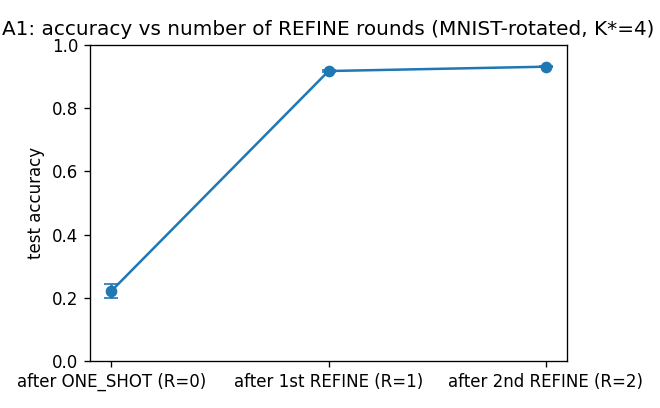
\includegraphics[width=0.7\textwidth]{Figures/srfca/ablation_A1.png}
\caption{A1: SR-FCA test accuracy on MNIST-rotated as a function of the number of REFINE rounds $R$. Three seeds, mean $\pm$ std.}\label{fig:ablation-A1}
\end{figure}

\paragraph{Pattern: large jump at $R = 1$, smaller bump at $R = 2$.} ONE\_SHOT alone reaches $22.25 \pm 2.20\,\%$ -- the cluster \emph{assignment} is already perfect at $R = 0$ (misclustering is zero on every seed), but the cluster \emph{models} have only been trained for the brief $T_0$ local-warmup pass, so per-client test accuracy is barely above chance for 10-class MNIST. One full REFINE round trains each cluster model for $T = 280$ rounds of TrimmedMeanGD with $E = 2$ local epochs per round, and accuracy jumps to $91.72 \pm 0.17\,\%$. A second REFINE round buys another $1.36$ percentage points to $93.08 \pm 0.09\,\%$, with smaller variance.

\paragraph{Comparison with paper's Table~5.} The qualitative pattern matches the paper exactly. Paper Table~5 reports for MNIST-rotated: after ONE\_SHOT $85.55 \pm 0.19$, after 1st REFINE $91.63 \pm 0.12$, after 2nd REFINE $91.66 \pm 0.13$ -- a large jump from ONE\_SHOT to the first REFINE and a small bump from the first to the second. Our progression $22.25 \to 91.72 \to 93.08$ shows the same shape with a much sharper $R = 0 \to R = 1$ jump (because our ONE\_SHOT-only accuracy is much lower; see below) and a slightly larger $R = 1 \to R = 2$ bump. Our $93.08\,\%$ at $R = 2$ also matches the SR-FCA row of Table~\ref{tab:main-acc} (five seeds).

\paragraph{Why the cluster assignment is already perfect at $R = 0$.} This is the most useful finding of the ablation: \emph{the value of REFINE in our setting is almost entirely about training the cluster models, not about correcting the clustering}. ONE\_SHOT recovers $K^\star = 4$ with zero misclustering on every seed, and RECLUSTER and MERGE are no-ops in subsequent rounds (no client gets reassigned, no clusters get merged). What REFINE actually does is run TrimmedMeanGD inside each cluster, which is where the accuracy comes from. The robustness margin of TrimmedMeanGD is not exercised because there are no mis-clustered clients to be robust against. This is the empirical analogue of Theorem~4.14: under the assumptions of clean separation, $R = 1$ already gives exact clustering, and additional REFINE rounds only sharpen the per-cluster models.

\section{New dataset: Fashion-MNIST rotated}\label{sec:fashion}

We use Fashion-MNIST with the same four-angle rotation split ($K^\star = 4$), the same MLP, and the same full-scale SR-FCA hyperparameters. Five seeds, SR-FCA only.

\begin{table}[h]
\centering
\small
\begin{tabular}{lcc}
\toprule
Method & Test acc (\%) & Misclust. \\
\midrule
\textbf{SR-FCA} & $\mathbf{83.96 \pm 0.30}$ & $\mathbf{0.00}$ \\
\bottomrule
\end{tabular}
\caption{Fashion-MNIST rotated ($K^\star = 4$). Five seeds, full-scale SR-FCA configuration. The paper does not report Fashion-MNIST numbers; this is a self-designed extension.}\label{tab:fashion}
\end{table}

\begin{figure}[h]
\centering
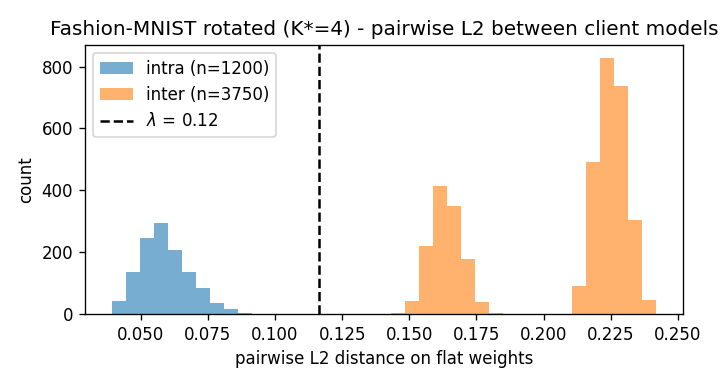
\includegraphics[width=0.49\textwidth]{Figures/srfca/pairwise_hist_fashion_mnist.png}
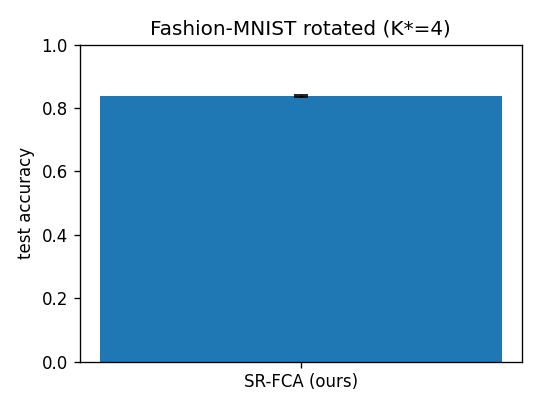
\includegraphics[width=0.49\textwidth]{Figures/srfca/fashion_mnist_bar.png}
\caption{Fashion-MNIST rotated, five seeds, SR-FCA full-scale configuration. Left: pairwise-$\ell_2$ histogram between locally-trained client models, seed $0$. Right: SR-FCA test accuracy across seeds.}\label{fig:fashion-bar}
\end{figure}

\paragraph{What this experiment tests.} Fashion-MNIST is a harder image distribution than MNIST: it has more visually-similar inter-class pairs (pullover/coat, sandal/sneaker) and a smaller signal-to-noise ratio per pixel. The question is whether SR-FCA's clustering primitive -- pairwise $\ell_2$ on locally-trained models -- still produces a clean valley between intra- and inter-cluster modes when the per-client local optimum is noisier.

\paragraph{Result.} SR-FCA reaches $83.96 \pm 0.30\,\%$ test accuracy on Fashion-MNIST rotated and recovers $K^\star = 4$ with zero misclustering on every seed. This is approximately $9$ percentage points below the corresponding MNIST-rotated number ($93.02\,\%$), in line with the per-class supervised gap between MNIST and Fashion-MNIST under the same MLP architecture. The reduction is in \emph{absolute} accuracy, not in cluster-recovery quality: the pairwise-distance histogram (Figure~\ref{fig:fashion-bar}, left) remains cleanly bimodal, and ONE\_SHOT picks $K^\star = 4$ on every seed without intervention. The seed-to-seed standard deviation ($\pm 0.30$) is comparable to the MNIST runs, so the additional intrinsic difficulty of Fashion-MNIST does not destabilise SR-FCA's clustering decisions.

\section{Summary of Part B}\label{sec:part-b-summary}

We reproduce SR-FCA on the paper's two simulated MNIST splits at the paper's actual full-scale configuration. The headline numbers -- $93.02 \pm 0.17\,\%$ rotated and $92.95 \pm 0.18\,\%$ inverted, against the paper's $91.66 \pm 0.13$ and $92.03 \pm 0.30$ -- land slightly above the paper, with zero misclustering on every seed and $K^\star$ recovered correctly on every seed of every experiment. The five baseline methods (Local, Global, CFL, LOCAL-KMeans, IFCA) are quoted from Tables~2 and~3 of~\parencite{vardhan2024srfca} as reference points; this scope decision is documented in \S\ref{sec:repro-scope}. The A1 ablation reproduces the paper's Table~5 pattern of accuracy jumps ($22.25 \to 91.72 \to 93.08\,\%$ across $R = 0/1/2$) and exposes the underlying mechanism: ONE\_SHOT already picks the right clustering on clean simulated data, and REFINE's effect is almost entirely about training the per-cluster models rather than correcting the assignment. The Fashion-MNIST evaluation ($83.96 \pm 0.30\,\%$, zero misclustering) extends the method to a dataset the authors did not study and confirms the qualitative behaviour transfers.
